%% 第二章--chapter2.tex
\chapter{示例}\echapter{Examples}\label{chap:CodeIntro}
\section{公式与数学类环境}\esection{Formulas and Math Environments}\label{subsec:eqandmath}
公式分为编号和不编号的两类。可以使用\env{equation}环境为公式编号。
\begin{equation}\label{eq:gougu}
	x_{1,2}=\frac{-b \pm \sqrt{b^2-4ac}}{2a}.
\end{equation}
加上 \cs{label},就能使用 \cs{ref}或 \cs{eqref}引用了。
代入式~\ref{eq:gougu},可解得式~\eqref{eq:gougu}。

不编号的公式使用 \env{equation*} 环境。
\begin{equation*}
	\int_{-\infty}^{+\infty}\frac{1}{\sqrt{2\uppi}\sigma}		% 直立的 π
	\mathrm{e}^{-\tfrac{(x-\mu)^2}{2\sigma^2}} \,\mathrm{d}x =1
\end{equation*}

行内公式可套以美元符号 \verb+$  $+,如 $f(x)=ax^2+bx+c$.
对于上述 \env{equation*} 环境中的公式(即行间公式),可套以双美元符号 \verb+$$  $$+
或 \verb+\[   \]+。
但是并不建议使用前者,因其在 \LaTeX\ 中并没有完整的重定义,有可能会在某些命令上失效。

关于公式的命令可以参考 \pkg{amsmath} 宏包说明文档,中译可参考 \href{http://static.latexstudio.net/article/2019/0204/amsmath-guide-zh-cn.pdf}{amsmath 包使用手册};
%除此之外可参考 \href{http://media.cism.it/attachments/ch8.pdf}{Higher Mathematics}。
还有一些在线网站,如 \href{https://latexlive.com/}{latexlive} 不仅能够即时预览,还提供了图像与手写识别系统。
以下举几个例子来展示最常见的用法:

由$\cos 2x=\cos^2x-\sin^2x$ ,	% 函数
则$\Vector{n}=a\Vector{x}+b\Vector{y}+c\Vector{z}.$	% 自定义向量,区别于\vec。见 mycfg.sty
又因$\mathcal{M}\in \mathbb{R}$,			% 字母样式
于是
\[
	\int_a^b f(t)\,\mathrm{d}t = \iint\limits_S g(x,y)\,\mathrm{d}x\mathrm{d}y
	= \iiint\nolimits_D\, \mathrm{d}h.	% 积分号及角标
\]
得
\[\lim_{n \to \infty}\sum_{i=1}^n{\frac{1}{n}}\sin\frac{k}{n}.\]	% 极限、无穷、求和
故
\begin{equation}\label{eq:res}
	\oint_{\gamma}f(z)\,\mathrm{d}z=2\uppi\symbfit{i}\sum^n_{k=1}\mathrm{I}(\gamma,a_k)\mathrm{Res}(f,a_k).
\end{equation}

若要公式多行对齐,可以使用 \env{align} 环境。下面的例子在等号处对齐:
\begin{align}
	x^2 + y^2 & = 1            \\
	x         & = \sqrt{1-y^2} \\\text{and also }
	y         & =\sqrt{1-x^2}
\end{align}
这会对每一行的公式进行编号。若在 \env{equation} 环境中嵌套 \env{aligned} 环境,加上参数[b]
可以达到多行对齐但只对最后一个式子编号的效果:
\begin{equation}
	\begin{aligned}[b]
		(a + b)^3   & = (a + b) (a + b)^2         \\
					& = (a + b)(a^2 + 2ab + b^2)  \\
					& = a^3 + 3a^2b + 3ab^2 + b^3
	\end{aligned}
\end{equation}

模板使用 \pkg{amsthm} 宏包预定义了部分与数学相关的环境,格式及编号如下:
\begin{axiom}
	这是一条axiom,使用\env{axiom}环境。
\end{axiom}
\begin{theorem}[某某定理]   % []内为可选参数
	这是一条theorem,使用\env{theorem}环境。
\end{theorem}
\begin{corollary}[一条推论]\label{cor:cor1}
	这是一条corollary,使用\env{corollary}环境。
\end{corollary}
\begin{proof}
	这是一条proof,使用\env{proof}环境。
	\[
		\Matrix{A}=\begin{bmatrix}
			a_{11} & \cdots  & a_{1n} \\
			\vdots & \ddots & \vdots \\
			0      & \cdots & a_{nn}
		\end{bmatrix}_{n\times n}
	\]

	在证明的最后一行会加上证毕符号,若其位置不合理则需加上命令 \cs{qedhere}。
	综上所述,推论 \ref{cor:cor1} 成立。
\end{proof}
\begin{remark}
	这是一条remark,使用\env{remark}环境。
\end{remark}
\begin{assumption}
	这是一条assumption,使用\env{assumption}环境。
\end{assumption}
\begin{definition}
	这是一条definition,使用\env{definition}环境。
\end{definition}
\begin{property}
	这是一条property,使用\env{property}环境。
\end{property}
\begin{proposition}
	这是一条proposition,使用\env{proposition}环境。
\end{proposition}
\begin{lemma}
	这是一条lemma,使用\env{lemma}环境。
\end{lemma}

以上是模板已经定义了的数学类环境,但也能自定义。
如:
\newtheorem{tale}{传说}[chapter]	% 计数与章编号相关
\begin{tale}[山经]	  % []内为可选参数
	精卫衔微木,将以填沧海。
\end{tale}
\begin{tale}[海经]
	刑天舞干戚,猛志固常在。
\end{tale}


\section{代码}\esection{Codes}\label{subsec:code}
若要在文中插入代码,简单的代码可以使用原文照列命令~\verb+\verb+或~\verb*@\verb*@,
比如~\verb-i++-、\verb*|int main|,二者区别在于,带*号的将展示代码中的空格。
如果插入代码块,可使用环境\env{lstlisting},且可以有如下选择:
\subsection{直接在 \LaTeX\ 中书写代码}\esubsection{Writing Codes in \LaTeX}
\begin{lstlisting}[language=C++,caption=Hello World!,label=code:HelloWorld]
/* Hello World C++ */
#include<iostream>
using namespace std;
/*****   main function	*****/
int main()
{
	cout<<"Hello World!"<<endl;		@*//Print "Hello World!", I'm \LaTeX{}!@*
	return 0;
}
\end{lstlisting}
\subsection{引用代码文件}\esubsection{Inputing files into \LaTeX}
源代码存放于 \file{code/} 文件夹里,直接调用即可。
\lstinputlisting[
	language=C++,
	caption=你好,世界!,
	label=code:HelloWorld2
]{code/helloworld.cpp}

模板按照《规范》以 Times New Roman 字体书写代码。
代码的关键字以粗体标出,而注释(西文)使用斜体。
模板载入文档类时的 \opt{submit} 选项将关闭代码颜色。

代码 \ref{code:HelloWorld} 展示了如何从代码块中临时返回到 \LaTeX\ 中。

\section{化学类}\esection{Chemistry}
模板加载了 \pkg{mhchem} 宏包,方便了化学(方程)式的书写。
使用命令 \cs{ce}\marg{formula} 把化学(方程)式括起来。
\subsection{简单化学式}\esubsection{Simple Chemical Formulas}
\begin{table}[H]
	\centering
	\begin{tabular}{llllll}
		\ce{H2O}    & \ce{Sb2O3}  & \ce{KCr(SO4)2.12H2O} & \ce{CrO4^2-}                & \ce{[AgCl2]-}              & \ce{^{0}_{-1}M^{-}} \\
		\ce{$n$H2O} & \ce{H2(aq)} & \ce{KCr(SO4)2*12H2O} & \ce{Fe(CN)_{$\frac{6}{2}$}} & \ce{$cis${-}[PtCl2(NH3)2]} & \ce{\alpha-Al2O3}   \\
	\end{tabular}
\end{table}
\subsection{含键化学式}\esubsection{Chemical Formulas With Bonds}
\begin{table}[H]
	\centering
	\begin{tabular}{llll}
		\ce{A-B=C#D}                           & \ce{A\bond{-}B\bond{=}C\bond{#}D} & \ce{A\bond{1}B\bond{2}C\bond{3}D} & \ce{A\bond{~}B\bond{~-}C} \\
		\ce{A\bond{~--}B\bond{~=}C\bond{-~-}D} & \ce{A\bond{...}B\bond{....}C}     & \ce{A\bond{->}B\bond{<-}C}        &                           \\
	\end{tabular}
\end{table}
\subsection{化学方程式}\esubsection{Chemical Equations}
\begin{table}[H]
	\centering
	\begin{tabular}{llll}
		\ce{A ->[H2O] B} & \ce{A <=>[{上方文字}][{text below}] B} & \ce{A ->[$x$][$x_i$] B} & \ce{A v B (v) -> C ^ D (^)} \\
	\end{tabular}
\end{table}
\subsection{其他}\esubsection{Others}
\begin{itemize}
	\item 标注(可能对 CJK 文字不支持):
			\ce{Zn^2+
			<=>[+ 2OH-][+ 2H+]
			$\underset{\text{amphoteres Hydroxid}}{\ce{Zn(OH)2 v}}$
			<=>[+ 2OH-][+ 2H+]
			$\underset{\text{Hydroxozikat}}{\ce{[Zn(OH)4]^2-}}$
			}
	\item 对于化学方程式等的编号,与数学方程相似:
			$$\ce{2H2O ->[{electrify}] 2H2 ^ + O2 ^}$$
			\begin{equation}
					K^\ominus  = \ce{\frac{[Hg^2+][Hg]}{[Hg2^2+]}}
			\end{equation}
\end{itemize}

至于有机化学的结构式等,尽管有一些宏包可以绘制,但使用图片插入可能是一个更好
的选择。

\section{文献引用和参考文献}\esection{Citing and Bibliography}\label{sec:bib}
模板使用 \cs{cite}\marg{CiteKey}命令实现上标、方括号以“顺序编码制”引用参考文献,
这是学校《规范》的要求。一个例子。\cite{abbott2016observation}而使用
\cs{nocite}\marg{CiteKey}命令则指明不引用但需要列出的参考文献。\nocite{*}

同一处引用多个文献时,应将各篇文献的引用标签一同写在 \cs{cite} 命令中,
并以西文逗号“,”分隔各标签。所产生的样式为:当在同一处引用两篇参考文献时,
引用序号将以西文逗号分隔;
当多余两篇且连续时,将标示起止序号并以短划线相连。这\cite{texbook,latexrumen}
又是\cite{texbook,latexrumen,gbt7714-2005}一个例子。\cite{abbott2016observation,texbook,latexrumen,buctthesis}

关于 \file{thesisbib.bib} 文件的编辑,
可以使用\href{http://scholar.google.com.cn/}{谷歌学术}\footnote{亦可以访问国内镜像站。}%
或\href{http://xueshu.baidu.com}{百度学术}两种方式(方法类似)将文献数据导入\BibTeX{}数据库,大致方法如下:
\begin{itemize}
	\item 在搜索框中搜索题目(或作者、DOI等),确定所引用的论文后点击“引用”;并在弹出框中,单击最下方“BibTeX”的链接,如图~\ref{fig:addbib};
	\item 在弹出的网页中复制所有代码至 \file{thesisbib.bib} 文件;
	\item 在论文中使用 \cs{cite} 命令引用相应的文献。
	\begin{table}
		\centering
		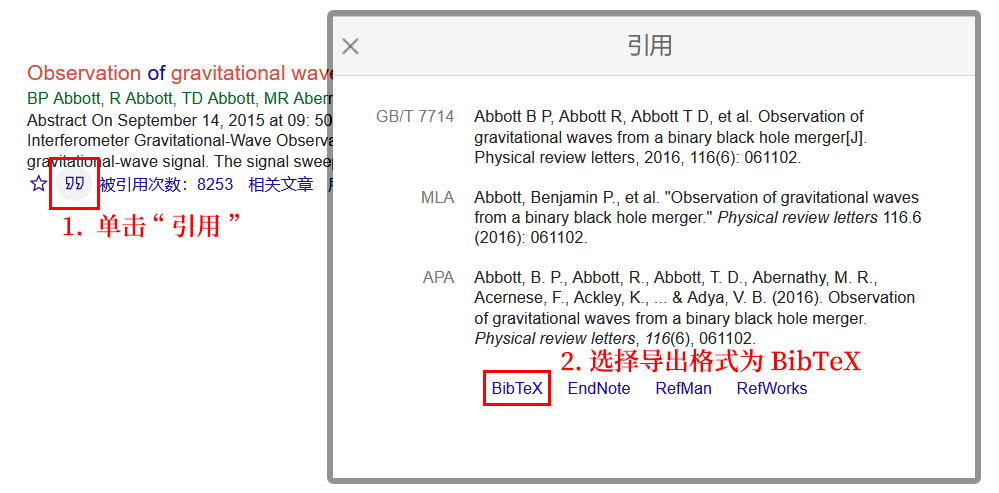
\includegraphics[width=.8\textwidth]{AddBib.png}
		\bicaption{使用谷歌学术导出参考文献数据}{How to export \BibTeX\ from Google Scholar}\label{fig:addbib}
	\end{table}
\end{itemize}

举个例子:经过图~\ref{fig:addbib} 所示步骤后,弹出的网页文本如下:
\begin{lstlisting}
@article{abbott2016observation,
	title={Observation of gravitational waves from a binary black hole merger},
	author={Abbott, Benjamin P and Abbott, Richard and %(省略)
	},
	journal={Physical review letters},
	volume={116},
	number={6},
	pages={061102},
	year={2016},
	publisher={APS}
}
	\end{lstlisting}
将以上内容复制进 \file{thesisbib.bib},在论文中使用
\cs{cite\{abbott2016observation\}}即可引用此文献。
这里的 “abbott2016observation”是该篇参考文献的引用标签,可以修改。
再来一个\cite{ashirov2008tetramerization} ,
网络上的资源引用\cite{buctthesis},等。

\section{其他}\esection{Others}\label{sec:other}

\subsection{脚注}\esubsection{Footnotes}\label{subsec:footnote}
本模板采用带圈数字脚注,计数跨页重置,使用命令 \cs{footnote}\marg{text}。
前方高能\footnote{我是可爱的脚注。}。

有些情况下(比如在表格环境、各种盒子内)使用 \cs{footnote}并不能正确生成脚注。
我们可以分两步进行,先使用 \cs{footnotemark}\oarg{text} 为脚注计数,
再在合适的位置用 \cs{footnotetext}\oarg{mark}\marg{text} 生成脚注。比如表~\ref{tab:ftnt1}。
\begin{table}[htb]
	\centering
	\bicaption{脚注示例1}{Example A of the footnotes}
	\label{tab:ftnt1}
	\begin{tabular}{llll}
		\hline
		人之初                & 性本善 & 性相近 & 习相远 \\
		苟\footnotemark 不教 & 性乃迁 & 教之道 & 贵以专 \\
		\hline
	\end{tabular}
\end{table}
\footnotetext{苟:如果。}

利用 \pkg{threeparttable} 宏包提供的 \env{threeparttable} 环境可以实现在表格底下写脚注,见表~\ref{tab:ftnt2}。

\begin{table}[htb]
\centering
\begin{threeparttable}
	\bicaption{脚注示例2}{Example B of the footnotes}\label{tab:ftnt2}
	\begin{tabular}{cccc}
		\toprule
		昔孟母	& 择邻处\tnote{*} & 子不学	& 断机杼\\
		\midrule
		窦燕山\tnote{$\dagger$}	& 有义方 & 教五子\tnote{$\ddagger$}	&名俱扬\\
		\bottomrule
	\end{tabular}
	\begin{tablenotes}\small
		\item [*] 脚注1。
		\item [$\dagger$] 脚注2。
		\item [$\ddagger$] 脚注3。
	\end{tablenotes}
\end{threeparttable}
\end{table}

\subsection{列表环境}\esubsection{Lists}\label{subsec:items}
本模板提供了三种列表环境:不编号的\env{itemize}、编号的\env{enumerate}
和使用关键字的\env{description}环境。在文档的中英文摘要部分分别展示了
基础的编号和不编号的列表环境;上面三种列表环境可以嵌套使用(至多四层),
且会自动处理不同层次的缩进和编号,如下所示:
\begin{itemize}
	\item 一条
	\item 次条
	\item 这一条可以分为\dots
		\begin{itemize}
			\item 子一条
		\end{itemize}
\end{itemize}
稍复杂一点的,如:
\begin{enumerate}
	\item 中文
		\begin{description}
			\item[文言文] 古代汉语
			\item[白话文] 现代汉语
				\begin{enumerate}
					\item 口语
						\begin{enumerate}
							\item 普通话
							\item 方言
						\end{enumerate}
					\item 书面语
				\end{enumerate}
		\end{description}
	\item English
\end{enumerate}

注意:一级编号列表环境最多罗列10条,否则标签会显示错误。
%,到第11条时,标签将从第10条的\ding{201}到第11条的\ding{202}
